% Options for packages loaded elsewhere
\PassOptionsToPackage{unicode}{hyperref}
\PassOptionsToPackage{hyphens}{url}
%
\documentclass[
]{article}
\usepackage{amsmath,amssymb}
\usepackage{lmodern}
\usepackage{iftex}
\ifPDFTeX
  \usepackage[T1]{fontenc}
  \usepackage[utf8]{inputenc}
  \usepackage{textcomp} % provide euro and other symbols
\else % if luatex or xetex
  \usepackage{unicode-math}
  \defaultfontfeatures{Scale=MatchLowercase}
  \defaultfontfeatures[\rmfamily]{Ligatures=TeX,Scale=1}
\fi
% Use upquote if available, for straight quotes in verbatim environments
\IfFileExists{upquote.sty}{\usepackage{upquote}}{}
\IfFileExists{microtype.sty}{% use microtype if available
  \usepackage[]{microtype}
  \UseMicrotypeSet[protrusion]{basicmath} % disable protrusion for tt fonts
}{}
\makeatletter
\@ifundefined{KOMAClassName}{% if non-KOMA class
  \IfFileExists{parskip.sty}{%
    \usepackage{parskip}
  }{% else
    \setlength{\parindent}{0pt}
    \setlength{\parskip}{6pt plus 2pt minus 1pt}}
}{% if KOMA class
  \KOMAoptions{parskip=half}}
\makeatother
\usepackage{xcolor}
\usepackage[margin=1in]{geometry}
\usepackage{color}
\usepackage{fancyvrb}
\newcommand{\VerbBar}{|}
\newcommand{\VERB}{\Verb[commandchars=\\\{\}]}
\DefineVerbatimEnvironment{Highlighting}{Verbatim}{commandchars=\\\{\}}
% Add ',fontsize=\small' for more characters per line
\usepackage{framed}
\definecolor{shadecolor}{RGB}{248,248,248}
\newenvironment{Shaded}{\begin{snugshade}}{\end{snugshade}}
\newcommand{\AlertTok}[1]{\textcolor[rgb]{0.94,0.16,0.16}{#1}}
\newcommand{\AnnotationTok}[1]{\textcolor[rgb]{0.56,0.35,0.01}{\textbf{\textit{#1}}}}
\newcommand{\AttributeTok}[1]{\textcolor[rgb]{0.77,0.63,0.00}{#1}}
\newcommand{\BaseNTok}[1]{\textcolor[rgb]{0.00,0.00,0.81}{#1}}
\newcommand{\BuiltInTok}[1]{#1}
\newcommand{\CharTok}[1]{\textcolor[rgb]{0.31,0.60,0.02}{#1}}
\newcommand{\CommentTok}[1]{\textcolor[rgb]{0.56,0.35,0.01}{\textit{#1}}}
\newcommand{\CommentVarTok}[1]{\textcolor[rgb]{0.56,0.35,0.01}{\textbf{\textit{#1}}}}
\newcommand{\ConstantTok}[1]{\textcolor[rgb]{0.00,0.00,0.00}{#1}}
\newcommand{\ControlFlowTok}[1]{\textcolor[rgb]{0.13,0.29,0.53}{\textbf{#1}}}
\newcommand{\DataTypeTok}[1]{\textcolor[rgb]{0.13,0.29,0.53}{#1}}
\newcommand{\DecValTok}[1]{\textcolor[rgb]{0.00,0.00,0.81}{#1}}
\newcommand{\DocumentationTok}[1]{\textcolor[rgb]{0.56,0.35,0.01}{\textbf{\textit{#1}}}}
\newcommand{\ErrorTok}[1]{\textcolor[rgb]{0.64,0.00,0.00}{\textbf{#1}}}
\newcommand{\ExtensionTok}[1]{#1}
\newcommand{\FloatTok}[1]{\textcolor[rgb]{0.00,0.00,0.81}{#1}}
\newcommand{\FunctionTok}[1]{\textcolor[rgb]{0.00,0.00,0.00}{#1}}
\newcommand{\ImportTok}[1]{#1}
\newcommand{\InformationTok}[1]{\textcolor[rgb]{0.56,0.35,0.01}{\textbf{\textit{#1}}}}
\newcommand{\KeywordTok}[1]{\textcolor[rgb]{0.13,0.29,0.53}{\textbf{#1}}}
\newcommand{\NormalTok}[1]{#1}
\newcommand{\OperatorTok}[1]{\textcolor[rgb]{0.81,0.36,0.00}{\textbf{#1}}}
\newcommand{\OtherTok}[1]{\textcolor[rgb]{0.56,0.35,0.01}{#1}}
\newcommand{\PreprocessorTok}[1]{\textcolor[rgb]{0.56,0.35,0.01}{\textit{#1}}}
\newcommand{\RegionMarkerTok}[1]{#1}
\newcommand{\SpecialCharTok}[1]{\textcolor[rgb]{0.00,0.00,0.00}{#1}}
\newcommand{\SpecialStringTok}[1]{\textcolor[rgb]{0.31,0.60,0.02}{#1}}
\newcommand{\StringTok}[1]{\textcolor[rgb]{0.31,0.60,0.02}{#1}}
\newcommand{\VariableTok}[1]{\textcolor[rgb]{0.00,0.00,0.00}{#1}}
\newcommand{\VerbatimStringTok}[1]{\textcolor[rgb]{0.31,0.60,0.02}{#1}}
\newcommand{\WarningTok}[1]{\textcolor[rgb]{0.56,0.35,0.01}{\textbf{\textit{#1}}}}
\usepackage{graphicx}
\makeatletter
\def\maxwidth{\ifdim\Gin@nat@width>\linewidth\linewidth\else\Gin@nat@width\fi}
\def\maxheight{\ifdim\Gin@nat@height>\textheight\textheight\else\Gin@nat@height\fi}
\makeatother
% Scale images if necessary, so that they will not overflow the page
% margins by default, and it is still possible to overwrite the defaults
% using explicit options in \includegraphics[width, height, ...]{}
\setkeys{Gin}{width=\maxwidth,height=\maxheight,keepaspectratio}
% Set default figure placement to htbp
\makeatletter
\def\fps@figure{htbp}
\makeatother
\setlength{\emergencystretch}{3em} % prevent overfull lines
\providecommand{\tightlist}{%
  \setlength{\itemsep}{0pt}\setlength{\parskip}{0pt}}
\setcounter{secnumdepth}{-\maxdimen} % remove section numbering
\ifLuaTeX
  \usepackage{selnolig}  % disable illegal ligatures
\fi
\IfFileExists{bookmark.sty}{\usepackage{bookmark}}{\usepackage{hyperref}}
\IfFileExists{xurl.sty}{\usepackage{xurl}}{} % add URL line breaks if available
\urlstyle{same} % disable monospaced font for URLs
\hypersetup{
  hidelinks,
  pdfcreator={LaTeX via pandoc}}

\author{}
\date{\vspace{-2.5em}}

\begin{document}

\hypertarget{reproducable-research-project-1}{%
\section{Reproducable Research, Project
1}\label{reproducable-research-project-1}}

\hypertarget{part-1-loading-and-preprocessing-the-data}{%
\subsection{Part 1: Loading and preprocessing the
data}\label{part-1-loading-and-preprocessing-the-data}}

Data found here:
\url{https://d396qusza40orc.cloudfront.net/repdata\%2Fdata\%2Factivity.zip}
Download data and unzip files into your working direcory Next, Load the
data into R:

\begin{Shaded}
\begin{Highlighting}[]
\FunctionTok{setwd}\NormalTok{(}\StringTok{"C:/Users/LindseyBehrens/OneDrive {-} Genective/Documents/R Working/Coursera"}\NormalTok{)}

\NormalTok{Data }\OtherTok{\textless{}{-}} \FunctionTok{read.csv}\NormalTok{(}\StringTok{"activity.csv"}\NormalTok{)}
\FunctionTok{head}\NormalTok{(Data)}
\end{Highlighting}
\end{Shaded}

\begin{verbatim}
##   steps       date interval
## 1    NA 2012-10-01        0
## 2    NA 2012-10-01        5
## 3    NA 2012-10-01       10
## 4    NA 2012-10-01       15
## 5    NA 2012-10-01       20
## 6    NA 2012-10-01       25
\end{verbatim}

Take a look at the Data:

\begin{Shaded}
\begin{Highlighting}[]
\FunctionTok{str}\NormalTok{(Data)}
\end{Highlighting}
\end{Shaded}

\begin{verbatim}
## 'data.frame':    17568 obs. of  3 variables:
##  $ steps   : int  NA NA NA NA NA NA NA NA NA NA ...
##  $ date    : chr  "2012-10-01" "2012-10-01" "2012-10-01" "2012-10-01" ...
##  $ interval: int  0 5 10 15 20 25 30 35 40 45 ...
\end{verbatim}

Notice that the `date' column is read as a character instead of a date.
Let's fix that:

\begin{Shaded}
\begin{Highlighting}[]
\NormalTok{Data}\SpecialCharTok{$}\NormalTok{date }\OtherTok{\textless{}{-}} \FunctionTok{as.Date}\NormalTok{(Data}\SpecialCharTok{$}\NormalTok{date)}
\FunctionTok{str}\NormalTok{(Data)}
\end{Highlighting}
\end{Shaded}

\begin{verbatim}
## 'data.frame':    17568 obs. of  3 variables:
##  $ steps   : int  NA NA NA NA NA NA NA NA NA NA ...
##  $ date    : Date, format: "2012-10-01" "2012-10-01" ...
##  $ interval: int  0 5 10 15 20 25 30 35 40 45 ...
\end{verbatim}

\hypertarget{part-2-what-is-mean-total-number-of-steps-taken-per-day}{%
\subsection{Part 2: What is mean total number of steps taken per
day?}\label{part-2-what-is-mean-total-number-of-steps-taken-per-day}}

We will ignore the missing values here. Lets fine the total number of
steps:

\begin{Shaded}
\begin{Highlighting}[]
\NormalTok{totalSteps }\OtherTok{\textless{}{-}} \FunctionTok{sum}\NormalTok{(Data}\SpecialCharTok{$}\NormalTok{steps, }\AttributeTok{na.rm =} \ConstantTok{TRUE}\NormalTok{)}
\NormalTok{totalSteps}
\end{Highlighting}
\end{Shaded}

\begin{verbatim}
## [1] 570608
\end{verbatim}

570608 total steps!

Lets look at the distribution in a histogram:

\begin{Shaded}
\begin{Highlighting}[]
\FunctionTok{library}\NormalTok{(ggplot2)}
\end{Highlighting}
\end{Shaded}

\begin{verbatim}
## Warning: package 'ggplot2' was built under R version 4.2.3
\end{verbatim}

\begin{Shaded}
\begin{Highlighting}[]
\NormalTok{Histogram }\OtherTok{\textless{}{-}} \FunctionTok{ggplot}\NormalTok{(Data, }\FunctionTok{aes}\NormalTok{(}\AttributeTok{x=}\NormalTok{steps)) }\SpecialCharTok{+}
    \FunctionTok{geom\_histogram}\NormalTok{(}\AttributeTok{binwidth=}\DecValTok{25}\NormalTok{)}
\NormalTok{Histogram}
\end{Highlighting}
\end{Shaded}

\begin{verbatim}
## Warning: Removed 2304 rows containing non-finite values (`stat_bin()`).
\end{verbatim}

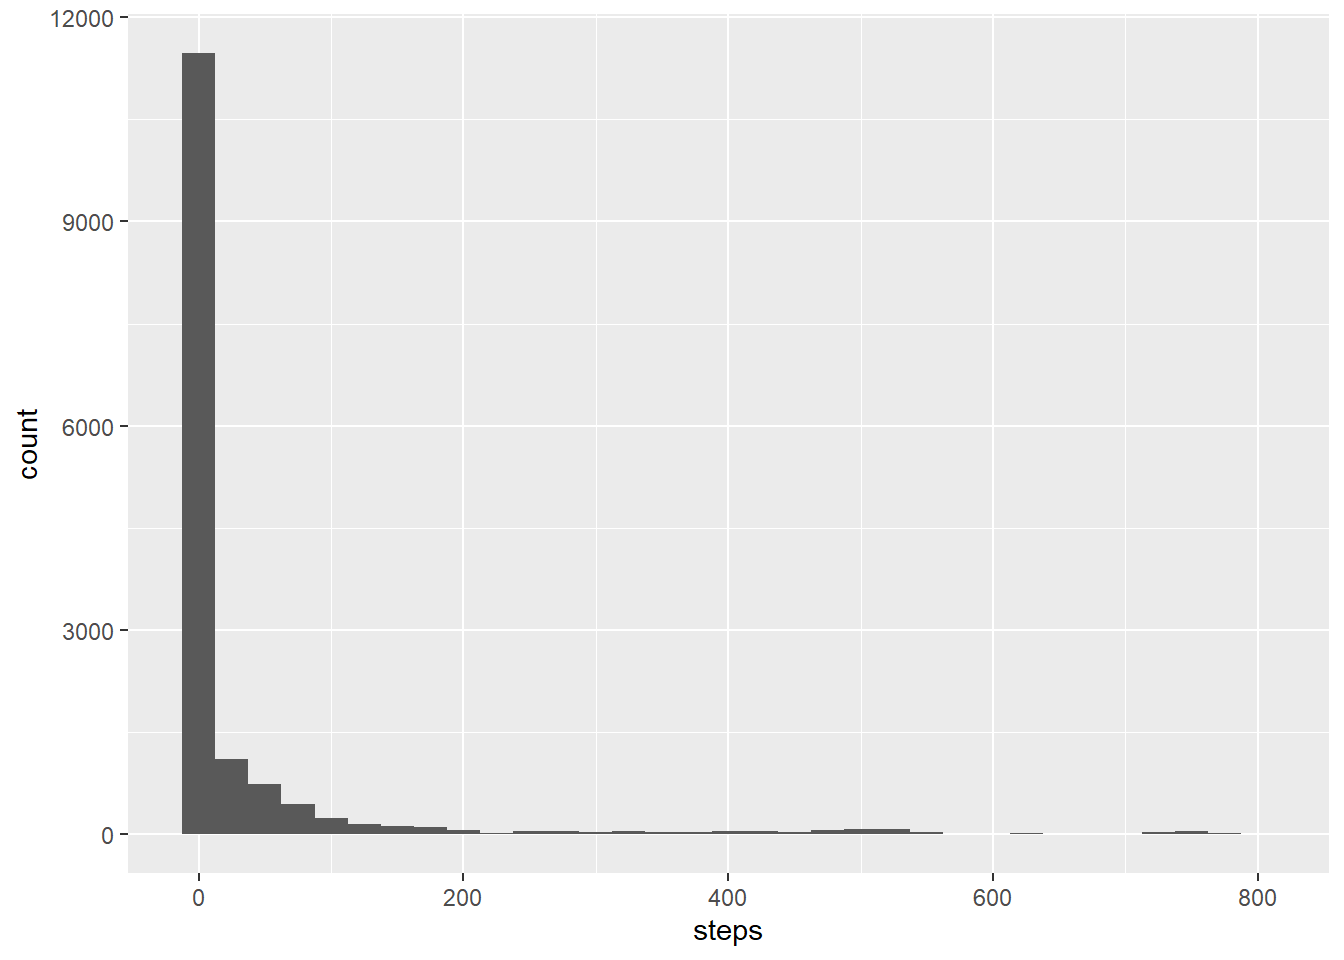
\includegraphics{PA1_template_files/figure-latex/HistogramSteps-1.pdf}

That's a lot of 0 steps.

Lets look at the mean and median number of steps:

\begin{Shaded}
\begin{Highlighting}[]
\NormalTok{meanSteps }\OtherTok{\textless{}{-}} \FunctionTok{mean}\NormalTok{(Data}\SpecialCharTok{$}\NormalTok{steps, }\AttributeTok{na.rm =} \ConstantTok{TRUE}\NormalTok{)}
\NormalTok{meanSteps}
\end{Highlighting}
\end{Shaded}

\begin{verbatim}
## [1] 37.3826
\end{verbatim}

\begin{Shaded}
\begin{Highlighting}[]
\NormalTok{medianSteps }\OtherTok{\textless{}{-}} \FunctionTok{median}\NormalTok{(Data}\SpecialCharTok{$}\NormalTok{steps, }\AttributeTok{na.rm =} \ConstantTok{TRUE}\NormalTok{)}
\NormalTok{medianSteps}
\end{Highlighting}
\end{Shaded}

\begin{verbatim}
## [1] 0
\end{verbatim}

Using this code we found that the mean number of steps was 37.3826 and
the median was 0 steps.

\hypertarget{part-3-what-is-the-average-daily-activity-pattern}{%
\subsection{Part 3: What is the average daily activity
pattern?}\label{part-3-what-is-the-average-daily-activity-pattern}}

Lets make a graph to look at the average number of steps in each
5-minute interval of the day

\begin{Shaded}
\begin{Highlighting}[]
\FunctionTok{library}\NormalTok{(dplyr)}
\end{Highlighting}
\end{Shaded}

\begin{verbatim}
## Warning: package 'dplyr' was built under R version 4.2.3
\end{verbatim}

\begin{verbatim}
## 
## Attaching package: 'dplyr'
\end{verbatim}

\begin{verbatim}
## The following objects are masked from 'package:stats':
## 
##     filter, lag
\end{verbatim}

\begin{verbatim}
## The following objects are masked from 'package:base':
## 
##     intersect, setdiff, setequal, union
\end{verbatim}

\begin{Shaded}
\begin{Highlighting}[]
\NormalTok{Averaged }\OtherTok{\textless{}{-}}\NormalTok{ Data }\SpecialCharTok{\%\textgreater{}\%}
  \FunctionTok{group\_by}\NormalTok{(interval) }\SpecialCharTok{\%\textgreater{}\%}
  \FunctionTok{summarize}\NormalTok{(}\AttributeTok{steps =} \FunctionTok{mean}\NormalTok{(steps, }\AttributeTok{na.rm =} \ConstantTok{TRUE}\NormalTok{))}


\NormalTok{AverageSteps }\OtherTok{\textless{}{-}} \FunctionTok{ggplot}\NormalTok{(Averaged, }\FunctionTok{aes}\NormalTok{(}\AttributeTok{y=}\NormalTok{steps, }\AttributeTok{x=}\NormalTok{ interval)) }\SpecialCharTok{+}
  \FunctionTok{geom\_line}\NormalTok{()}
\NormalTok{AverageSteps}
\end{Highlighting}
\end{Shaded}

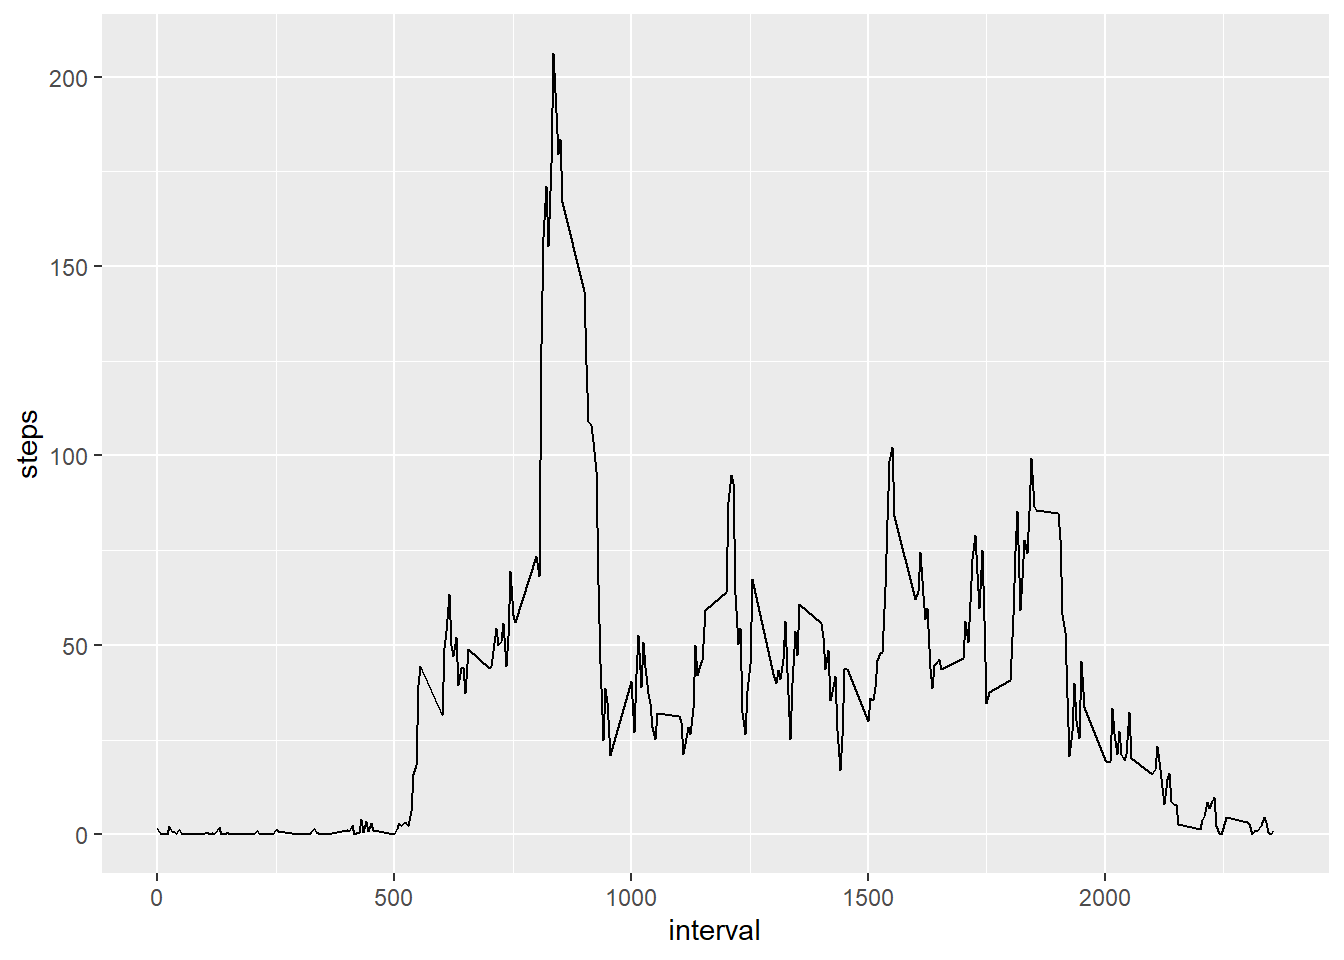
\includegraphics{PA1_template_files/figure-latex/intervals-1.pdf}

Now lets find the interval with the highest average number of setps

\begin{Shaded}
\begin{Highlighting}[]
\NormalTok{Highest }\OtherTok{\textless{}{-}} \FunctionTok{seq}\NormalTok{(}\AttributeTok{along=}\NormalTok{Averaged}\SpecialCharTok{$}\NormalTok{steps)[Averaged}\SpecialCharTok{$}\NormalTok{steps}\SpecialCharTok{==}\FunctionTok{max}\NormalTok{(Averaged}\SpecialCharTok{$}\NormalTok{steps)]}
\NormalTok{Averaged[Highest,]}
\end{Highlighting}
\end{Shaded}

\begin{verbatim}
## # A tibble: 1 x 2
##   interval steps
##      <int> <dbl>
## 1      835  206.
\end{verbatim}

Interval 835 with an average of 206 steps!

\hypertarget{part-4-imputing-missing-values}{%
\subsection{Part 4: Imputing missing
values}\label{part-4-imputing-missing-values}}

Note that there are a number of days/intervals where there are missing
values (coded as NA). The presence of missing days may introduce bias
into some calculations or summaries of the data.

Find the total number of rows with missing values:

\begin{Shaded}
\begin{Highlighting}[]
\NormalTok{Data\_No\_NA }\OtherTok{\textless{}{-}}\NormalTok{ Data[}\FunctionTok{complete.cases}\NormalTok{(Data), ]}
\NormalTok{NA\_count }\OtherTok{\textless{}{-}} \FunctionTok{nrow}\NormalTok{(Data) }\SpecialCharTok{{-}} \FunctionTok{nrow}\NormalTok{(Data\_No\_NA)}
\NormalTok{NA\_count}
\end{Highlighting}
\end{Shaded}

\begin{verbatim}
## [1] 2304
\end{verbatim}

There are 2304 missing values

Now we will fill the missing NA's with the median

\begin{Shaded}
\begin{Highlighting}[]
\FunctionTok{library}\NormalTok{(dplyr)}
\FunctionTok{library}\NormalTok{(tidyr)}
\end{Highlighting}
\end{Shaded}

\begin{verbatim}
## Warning: package 'tidyr' was built under R version 4.2.3
\end{verbatim}

\begin{Shaded}
\begin{Highlighting}[]
\NormalTok{Imputed\_Data }\OtherTok{\textless{}{-}}\NormalTok{ Data }\SpecialCharTok{\%\textgreater{}\%} 
  \FunctionTok{mutate}\NormalTok{(}\AttributeTok{steps =} \FunctionTok{replace\_na}\NormalTok{(steps,}\FunctionTok{median}\NormalTok{(steps, }\AttributeTok{na.rm =} \ConstantTok{TRUE}\NormalTok{)))}
\FunctionTok{nrow}\NormalTok{(Imputed\_Data) }\SpecialCharTok{==}  \FunctionTok{nrow}\NormalTok{(Data)}
\end{Highlighting}
\end{Shaded}

\begin{verbatim}
## [1] TRUE
\end{verbatim}

\begin{Shaded}
\begin{Highlighting}[]
\FunctionTok{head}\NormalTok{(Imputed\_Data)}
\end{Highlighting}
\end{Shaded}

\begin{verbatim}
##   steps       date interval
## 1     0 2012-10-01        0
## 2     0 2012-10-01        5
## 3     0 2012-10-01       10
## 4     0 2012-10-01       15
## 5     0 2012-10-01       20
## 6     0 2012-10-01       25
\end{verbatim}

After replacing the NA's with the median the data sets are the same
length and there are no more NA's

Now Lets make a histogram of the total number of steps taken each day

\begin{Shaded}
\begin{Highlighting}[]
\NormalTok{Histogram2 }\OtherTok{\textless{}{-}} \FunctionTok{ggplot}\NormalTok{(Imputed\_Data, }\FunctionTok{aes}\NormalTok{(}\AttributeTok{x=}\NormalTok{steps)) }\SpecialCharTok{+}
  \FunctionTok{geom\_histogram}\NormalTok{(}\AttributeTok{binwidth=}\DecValTok{25}\NormalTok{)}
\NormalTok{Histogram2}
\end{Highlighting}
\end{Shaded}

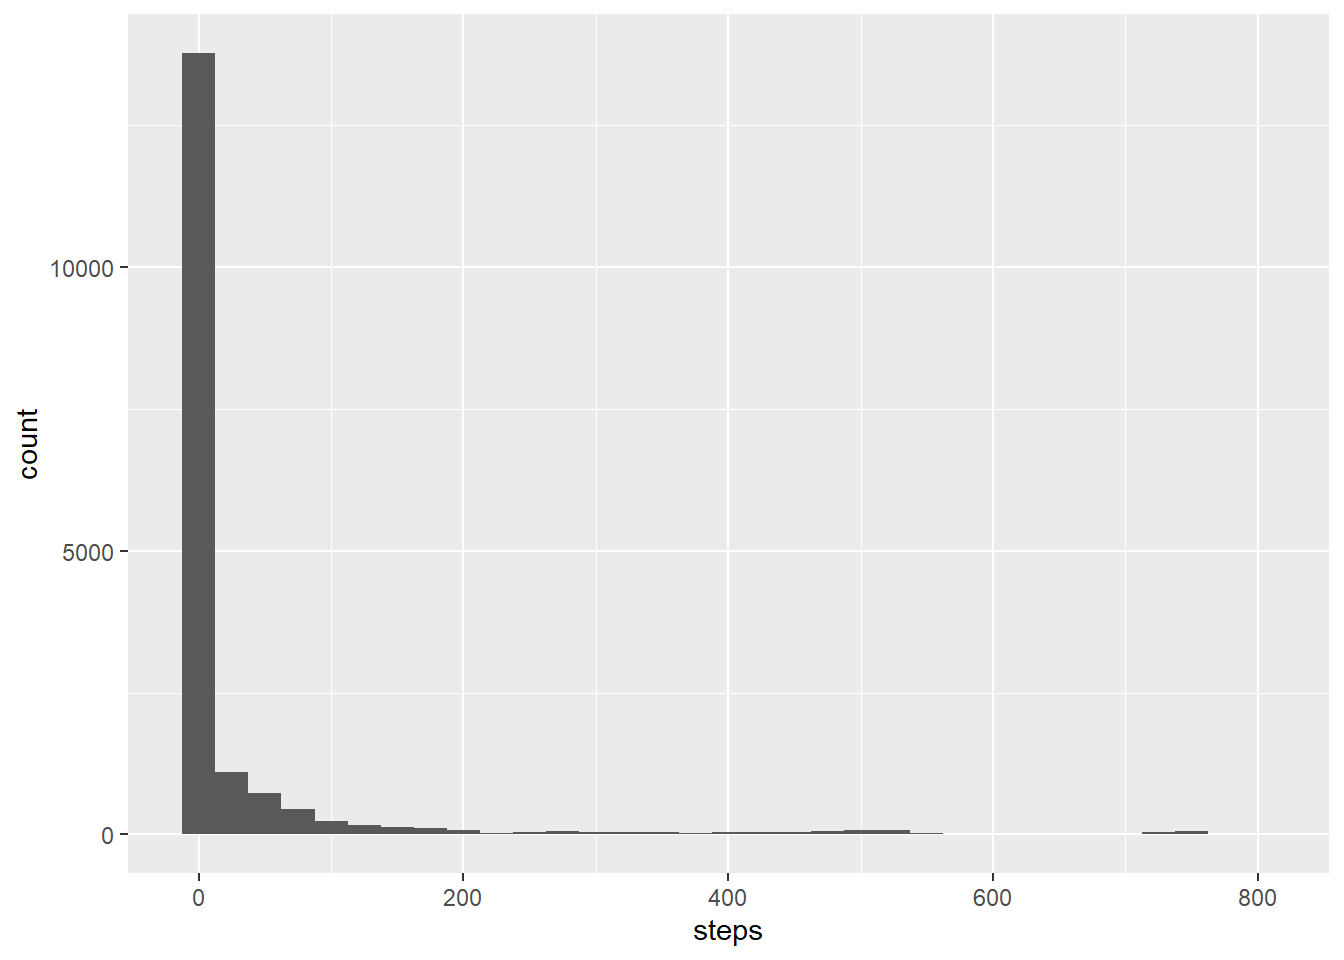
\includegraphics{PA1_template_files/figure-latex/Histogram2-1.pdf}

And look at the new mean and median

\begin{Shaded}
\begin{Highlighting}[]
\NormalTok{meanSteps2 }\OtherTok{\textless{}{-}} \FunctionTok{mean}\NormalTok{(Imputed\_Data}\SpecialCharTok{$}\NormalTok{steps, }\AttributeTok{na.rm =} \ConstantTok{TRUE}\NormalTok{)}
\NormalTok{meanSteps2}
\end{Highlighting}
\end{Shaded}

\begin{verbatim}
## [1] 32.47996
\end{verbatim}

\begin{Shaded}
\begin{Highlighting}[]
\NormalTok{medianSteps2 }\OtherTok{\textless{}{-}} \FunctionTok{median}\NormalTok{(Imputed\_Data}\SpecialCharTok{$}\NormalTok{steps, }\AttributeTok{na.rm =} \ConstantTok{TRUE}\NormalTok{)}
\NormalTok{medianSteps2}
\end{Highlighting}
\end{Shaded}

\begin{verbatim}
## [1] 0
\end{verbatim}

Do these values differ from the estimates from the first part of the
assignment? The mean is slightly lower and the median is the same.

\begin{Shaded}
\begin{Highlighting}[]
\NormalTok{meanSteps}
\end{Highlighting}
\end{Shaded}

\begin{verbatim}
## [1] 37.3826
\end{verbatim}

\begin{Shaded}
\begin{Highlighting}[]
\NormalTok{meanSteps2}
\end{Highlighting}
\end{Shaded}

\begin{verbatim}
## [1] 32.47996
\end{verbatim}

\begin{Shaded}
\begin{Highlighting}[]
\NormalTok{medianSteps}
\end{Highlighting}
\end{Shaded}

\begin{verbatim}
## [1] 0
\end{verbatim}

\begin{Shaded}
\begin{Highlighting}[]
\NormalTok{medianSteps2}
\end{Highlighting}
\end{Shaded}

\begin{verbatim}
## [1] 0
\end{verbatim}

What is the impact of imputing missing data on the estimates of the
total daily number of steps?

\begin{Shaded}
\begin{Highlighting}[]
\NormalTok{totalSteps2 }\OtherTok{\textless{}{-}} \FunctionTok{sum}\NormalTok{(Imputed\_Data}\SpecialCharTok{$}\NormalTok{steps, }\AttributeTok{na.rm =} \ConstantTok{TRUE}\NormalTok{)}
\NormalTok{totalSteps2}
\end{Highlighting}
\end{Shaded}

\begin{verbatim}
## [1] 570608
\end{verbatim}

\begin{Shaded}
\begin{Highlighting}[]
\NormalTok{totalSteps}
\end{Highlighting}
\end{Shaded}

\begin{verbatim}
## [1] 570608
\end{verbatim}

The same! The median was 0.

\hypertarget{part-5-are-there-differences-in-activity-patterns-between-weekdays-and-weekends}{%
\subsection{Part 5: Are there differences in activity patterns between
weekdays and
weekends?}\label{part-5-are-there-differences-in-activity-patterns-between-weekdays-and-weekends}}

Create a new factor variable in the dataset with two levels indicating
whether a given date is a weekday or weekend day.

\begin{Shaded}
\begin{Highlighting}[]
\NormalTok{Imputed\_Data}\SpecialCharTok{$}\NormalTok{Weekday }\OtherTok{\textless{}{-}} \FunctionTok{weekdays}\NormalTok{(Imputed\_Data}\SpecialCharTok{$}\NormalTok{date)}
\NormalTok{Day }\OtherTok{\textless{}{-}} \FunctionTok{c}\NormalTok{(}\StringTok{"Monday"}\NormalTok{, }\StringTok{"Tuesday"}\NormalTok{, }\StringTok{"Wednesday"}\NormalTok{, }\StringTok{"Thursday"}\NormalTok{, }\StringTok{"Friday"}\NormalTok{)}
\NormalTok{End }\OtherTok{\textless{}{-}} \FunctionTok{c}\NormalTok{(}\StringTok{"Saturday"}\NormalTok{, }\StringTok{"Sunday"}\NormalTok{)}

\NormalTok{Imputed\_Data}\SpecialCharTok{$}\NormalTok{Weekend }\OtherTok{\textless{}{-}}\NormalTok{  Imputed\_Data}\SpecialCharTok{$}\NormalTok{Weekday }\SpecialCharTok{\%in\%}\NormalTok{ End}
\NormalTok{Imputed\_Data }\OtherTok{\textless{}{-}}\NormalTok{ Imputed\_Data }\SpecialCharTok{\%\textgreater{}\%}
  \FunctionTok{mutate}\NormalTok{(}\AttributeTok{DayClass =} \FunctionTok{case\_when}\NormalTok{(}
\NormalTok{    Weekend }\SpecialCharTok{==} \ConstantTok{TRUE} \SpecialCharTok{\textasciitilde{}} \StringTok{"Weekend"}\NormalTok{,}
\NormalTok{    Weekend }\SpecialCharTok{==} \ConstantTok{FALSE} \SpecialCharTok{\textasciitilde{}} \StringTok{"Weekday"}
\NormalTok{  ))}

\FunctionTok{head}\NormalTok{(Imputed\_Data)}
\end{Highlighting}
\end{Shaded}

\begin{verbatim}
##   steps       date interval Weekday Weekend DayClass
## 1     0 2012-10-01        0  Monday   FALSE  Weekday
## 2     0 2012-10-01        5  Monday   FALSE  Weekday
## 3     0 2012-10-01       10  Monday   FALSE  Weekday
## 4     0 2012-10-01       15  Monday   FALSE  Weekday
## 5     0 2012-10-01       20  Monday   FALSE  Weekday
## 6     0 2012-10-01       25  Monday   FALSE  Weekday
\end{verbatim}

Make a time series plot of the 5-minute interval and the average number
of steps taken, averaged across all weekday days or weekend days

\begin{Shaded}
\begin{Highlighting}[]
\NormalTok{Classes }\OtherTok{\textless{}{-}} \FunctionTok{unique}\NormalTok{(Imputed\_Data}\SpecialCharTok{$}\NormalTok{DayClass)}
\NormalTok{Averaged2 }\OtherTok{\textless{}{-}} \FunctionTok{data.frame}\NormalTok{(}\FunctionTok{matrix}\NormalTok{(}\AttributeTok{ncol=}\DecValTok{3}\NormalTok{, }\AttributeTok{nrow=}\DecValTok{0}\NormalTok{))}
\ControlFlowTok{for}\NormalTok{ (Class }\ControlFlowTok{in}\NormalTok{ Classes) \{}
\NormalTok{  set }\OtherTok{\textless{}{-}} \FunctionTok{subset}\NormalTok{(Imputed\_Data, DayClass }\SpecialCharTok{==}\NormalTok{ Class)}
\NormalTok{  Average }\OtherTok{\textless{}{-}}\NormalTok{ set }\SpecialCharTok{\%\textgreater{}\%}
    \FunctionTok{group\_by}\NormalTok{(interval) }\SpecialCharTok{\%\textgreater{}\%}
    \FunctionTok{summarize}\NormalTok{(}\AttributeTok{steps =} \FunctionTok{mean}\NormalTok{(steps, }\AttributeTok{na.rm =} \ConstantTok{TRUE}\NormalTok{))}
\NormalTok{  Average}\SpecialCharTok{$}\NormalTok{DayClass }\OtherTok{\textless{}{-}}\NormalTok{ Class}
\NormalTok{  Averaged2 }\OtherTok{\textless{}{-}} \FunctionTok{rbind}\NormalTok{(Averaged2, Average)}
\NormalTok{\}}

\NormalTok{AverageSteps2 }\OtherTok{\textless{}{-}} \FunctionTok{ggplot}\NormalTok{(Averaged2, }\FunctionTok{aes}\NormalTok{(}\AttributeTok{y=}\NormalTok{steps, }\AttributeTok{x=}\NormalTok{ interval)) }\SpecialCharTok{+}
  \FunctionTok{geom\_line}\NormalTok{() }\SpecialCharTok{+}
  \FunctionTok{facet\_grid}\NormalTok{( }\SpecialCharTok{\textasciitilde{}}\NormalTok{ DayClass)}
\NormalTok{AverageSteps2}
\end{Highlighting}
\end{Shaded}

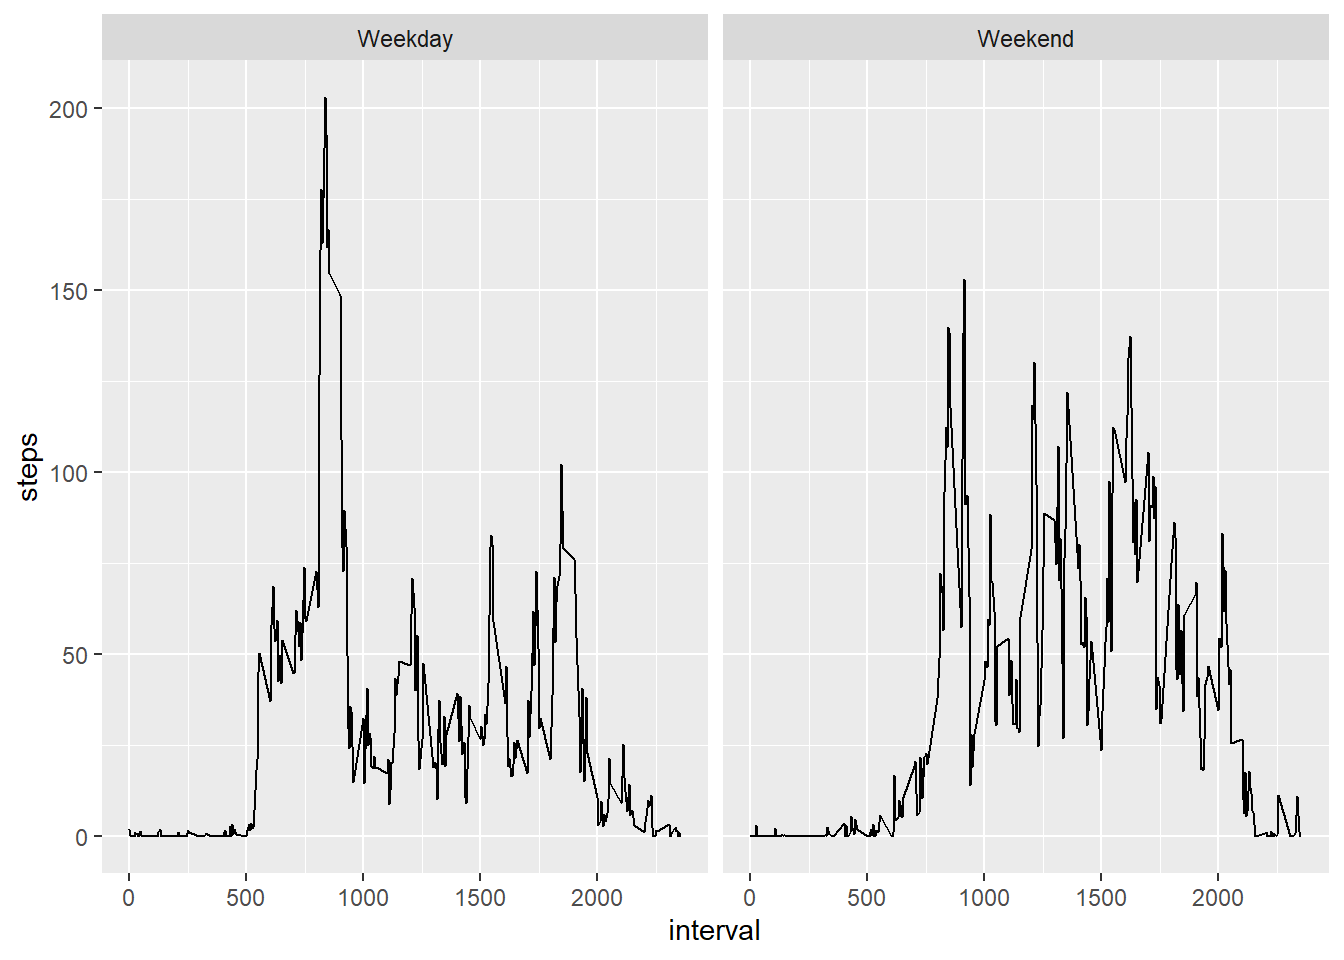
\includegraphics{PA1_template_files/figure-latex/weekdayGraph-1.pdf}

\end{document}
